
%(BEGIN_QUESTION)
% Copyright 2010, Tony R. Kuphaldt, released under the Creative Commons Attribution License (v 1.0)
% This means you may do almost anything with this work of mine, so long as you give me proper credit

Suppose you needed to control the temperature of an ``incubation'' vessel at a biopharmaceutical manufacturing facility, to ensure the bacteria were held at the correct temperature for optimum growth.  The vessel is heated by an electric heater, and the only controller you have available is one with a time-proportioning output (transistor).

Unfortunately, the controller's transistor is not able to directly handle the 240 volt AC power required by the heater, partly because of the voltage and current limitations of the transistor, and partly because an NPN transistor can only switch DC, not AC.

\vskip 50pt

$$\includegraphics[width=15.5cm]{i01488x01.eps}$$

\vskip 50pt

Sketch an ``interposing'' circuit between the controller and heating element that allows the controller to do its task.

\vfil 

\underbar{file i01488}
\eject
%(END_QUESTION)





%(BEGIN_ANSWER)

This is a graded question -- no answers or hints given!

%(END_ANSWER)





%(BEGIN_NOTES)

One of the most important general principles to keep in mind for this problem is the Law of Energy Conservation: {\it energy cannot be created or destroyed, but merely changed in form}.  Here, we are told the controller cannot handle either the voltage or the current necessary to energize a heating element.  This means no combination of passive components (capacitors, inductors, transformers, diodes, etc.) can ever boost the transistor's output power.  Instead, what the transistor can do is activate some kind of relay, which then switches 240 VAC power to the heating element.

Another important general principle to bear in mind is that transistors are not energy sources: one cannot simply connect the collector and emitter terminals of a transitor to a load device and expect that load device will receive power.  The transistor is merely an electronic {\it switch}: opening and closing to control direct current from some DC power source, which must be drawn in this circuit just like we need an AC power source to supply the heater.

Two alternative solutions are sketched here:

$$\includegraphics[width=15.5cm]{i01488x03.eps}$$

$$\includegraphics[width=15.5cm]{i01488x02.eps}$$

%INDEX% Control, proportional: time-proportioning output

%(END_NOTES)


